\documentclass{article}
\usepackage[a4paper, total={6.5in, 9in}]{geometry}
\usepackage{amsmath}
\usepackage{amssymb}
\usepackage{graphicx}
\usepackage{subfigure}
\usepackage{hyperref}
\usepackage{booktabs}
\usepackage{authblk}

\title{CSCI-SHU 360 Machine Learning\\
    Solution to homework 1}
\author{Josiah Li \texttt{yl11912@nyu.edu}}

\begin{document}
    \maketitle
\section{Simpson's Paradox}\label{sec:Simpson's Paradox} % (fold)

\subsection{} % (fold)
We use $ A $ to indicate that I win, and $ B $ to indicate that my friend wins.\\
We use $ M_i $ to indicate the player plays on the ith machine.
We have 
\begin{align*}
    P(A|M_1) = \frac{2}{5}&, P(A|M_2) = \frac{21}{104}\\
    P(B|M_1) = \frac{3}{10 }&, P(B|M_2) = \frac{1}{6}.
\end{align*}
Thus, on both machine 1 and machine 2, I am more likely to win.

\subsection{}
\begin{align*}
    P(A) &= \frac{40 + 210}{40 + 60 + 210 + 830} = \frac{25}{114} \\
    P(B) &= \frac{30 + 14}{30 + 70 + 14 + 70} = \frac{11 }{46}.
\end{align*}
Thus, my friend is more likely to win.

\subsection{} % (fold)
\begin{align*}
    P(A) &= P(A|M_1)P(M_1) + P(A|M_2)P(M_2) \\ 
    P(B) &= P(B|M_1)P(M_1) + P(B|M_2)P(M_2)
\end{align*}
Thus, when the $ P(M_i) $ increses, the total winning probability of player will get closer to the winning rate of machine i. \\ 
Thus, as I played much more rows on machine 2, and the overall winning rate on machine 2 is smaller than machin 1, my winning rate will get closer to the smaller winning rate(which is the winning rate of machine 2), and my friend's winning rate will be closer to the higher winning rate(which is the winning rate of machine 1), and that lead to the result that my winning rate is high on both machine, but the overall winning rate is lower than my friend.
% subsection  (end)
% subsubsection  (end)
% subsection  (end)
% section Simpson's Paradox (end)
\section{Matrix as Operations}\label{sec:Matrix as Operations} % (fold)
\subsection{} % (fold)
\begin{align*}
    a_1 = (1, 0)&, b_1 = (2, 0)\\
    a_2 = (0, 1)&, b_2 = (3, 2).
\end{align*}
Suppose $ W = \begin{bmatrix}
    W_{11} & W_{12} \\ W_{21} & W_{22}
\end{bmatrix}. $
We have
\begin{align*}
    b_1 &= Wa_1 = \begin{bmatrix}
        W_{11} & W_{12} \\ W_{21} & W_{22}
    \end{bmatrix}\begin{bmatrix}
    1 \\ 0 
    \end{bmatrix}=\begin{bmatrix}
    W_{11} \\ W_{21}
    \end{bmatrix} = \begin{bmatrix}
    2\\0
    \end{bmatrix}\\
    b_2 &= Wa_2 = \begin{bmatrix}
        W_{11 } & W_{12 } \\
        W_{21 } & W_{22}
    \end{bmatrix}\begin{bmatrix}
    0 \\1 
    \end{bmatrix} = \begin{bmatrix}
        W_{12} \\
        W_{22}
    \end{bmatrix} = \begin{bmatrix}
    3  \\ 2 
    \end{bmatrix}.
\end{align*}
Thus, we have
\begin{align*}
    W = \begin{bmatrix}
    2 & 3 \\
    0 & 2
    \end{bmatrix}.
\end{align*}
\subsection{} % (fold)
From $ \tan(\alpha  ) = 2 $, we have $ \sin(\alpha ) = \frac{2\sqrt{5}}{5} \text { and  } \cos(\alpha  ) = \frac{\sqrt5}{5} $(Suppose $ \alpha \in (0, \pi) $)\\
Moreover, we have the formula of the rotation matrix:
\begin{align*}
    R = \begin{bmatrix}
    \cos\theta  & \sin\theta  \\
    -\sin\theta  & \cos\theta
    \end{bmatrix}.
\end{align*} 
When $ \theta $ is the clockwise rotation angle. \\
Thus, $$ V = \begin{bmatrix}
\frac{\sqrt5 }{5} & \frac{2\sqrt{5}}{5} \\
-\frac{2\sqrt{5}}{5} & \frac{\sqrt 5 }{5}
\end{bmatrix} .$$
As $ \Sigma  $ scales the x-axis by a factor of 4 in two-dimensional space, the matrix is: $$ \Sigma = \begin{bmatrix}
4 & 0 \\
0 & 1
\end{bmatrix} .$$ \\
By using the same approach, we can get matrix $ U $. $ \tan(\beta) = \frac{1}{2}, \sin(\beta) = \frac{\sqrt{5}}{5}, \cos(\beta) = \frac{2 \sqrt{5}}{5} $,\\
And $$ U = \begin{bmatrix}
\frac{2 \sqrt{5}}{5} & -\frac{\sqrt{5}}{5} \\
\frac{\sqrt{5}}{5} & \frac{2 \sqrt{5}}{5}
\end{bmatrix} .$$
Multiplying three matrices together, we have:
\begin{align*}
    U\Sigma V &= \begin{bmatrix}
\frac{2 \sqrt{5}}{5} & -\frac{\sqrt{5}}{5} \\
\frac{\sqrt{5}}{5} & \frac{2 \sqrt{5}}{5}
\end{bmatrix}\begin{bmatrix}
4 & 0 \\
0 & 1
\end{bmatrix}  \begin{bmatrix}
\frac{\sqrt5 }{5} & \frac{2\sqrt{5}}{5} \\
-\frac{2\sqrt{5}}{5} & \frac{\sqrt 5 }{5}
\end{bmatrix} \\
              &= \begin{bmatrix}
\frac{2 \sqrt{5}}{5} & -\frac{\sqrt{5}}{5} \\
\frac{\sqrt{5}}{5} & \frac{2 \sqrt{5}}{5}
\end{bmatrix} \begin{bmatrix}
              \frac{4 \sqrt{5}}{5} & \frac{8 \sqrt{5}}{5} \\
              -\frac{2 \sqrt{5}}{5} & \frac{\sqrt{5}}{5}
              \end{bmatrix}\\
&= \begin{bmatrix}
2 & 3 \\
0 & 2
\end{bmatrix}\\
&= W.
\end{align*}
Thus, we have
\begin{align*}
    U\Sigma V = W.
\end{align*}
% subsection  (end)
% subsection  (end)         
\subsection{} % (fold)
We have
\[
    W = \begin{bmatrix}
    2 & 3 \\
    0 & 2
    \end{bmatrix}, W^T = \begin{bmatrix}
    2 & 0 \\
    3 & 2
    \end{bmatrix}
\]
Thus
\begin{align*}
    W^TW &= \begin{bmatrix}
    2 & 0 \\
    3 & 2
    \end{bmatrix}
    \begin{bmatrix}
    2 & 3 \\
    0 & 2
    \end{bmatrix} \\ 
    &= \begin{bmatrix}
    4 & 6 \\
    6 & 13 
    \end{bmatrix}
\end{align*}
% subsection  (end)
\begin{align*}
    det( W^TW - \lambda I ) &= det \left ( \begin{bmatrix}
    4-\lambda & 6 \\
    6 & 13- \lambda
    \end{bmatrix}\right )\\
    &= (13 - \lambda )(4 - \lambda ) - 36\\
    &= (\lambda - 16)(\lambda - 1)
\end{align*}
Thus, the eigenvalues and eigenvectors of $ W^TW $ are:
\begin{align*}
    \begin{cases}
        \lambda_1 = 1 , u_1 = \begin{bmatrix}
        -2 \\
        1 
        \end{bmatrix} \\
        \lambda_2 = 16, u_2 = \begin{bmatrix}
        1 \\
        2 
        \end{bmatrix}
    \end{cases}
\end{align*}
By applying the linear transformation $ W $, the unit circle is rotated clockwise by $ \alpha $ degrees, and then scales along x-axis by 4, finally, rotated counter-clockwise by $ \beta $ degrees. And this transformation results in a ellipse.
\subsection{} % (fold)
The determinant of $ W $ is $ det(W ) = 4 $. As in the previous transformation, we scaled along x-axis by 4, the semi-major axis is 4, and the semi-minor axis is 1. Thus, the area of the ellipse is $ 1 \times 4 \times \pi = 4\pi $ As the origin unit circle has an area of $ \pi  $, we came up with the hypothesis that the determinant shows the change of the area of a transformed shape. Using  a sentence to explain that $ det(AB ) = det(A )det(B ) $. Linear transformation $ AB $ means to perform first $ A $ and $ B $, and this means the total effect of the change of area will first be the effect of $ A  $, then multiplys the effect of $ B $, which in total is $ det(A )det(B) $.
% subsection  (end)
% section Matrix as Operations (end)
\section{Some Practices}\label{sec:Some Practices} % (fold)
\subsection{}\label{} % (fold)
As $ X $ is a discrete random variable, $ X^3 $ is also a discrete random variable. As $ Var(X^3) = \mathbb{E}[X^6] - (\mathbb{E}[X^3])^2 $ and $ Var(X^3) \geq 0 $, we can prove that:
\[
(\mathbb{E}[X^3])^2 \leq \mathbb{E}[X^6]
\]
% subsection  (end)
\subsection{} % (fold)
\begin{align*}
    (\mathbb{E}[X^3])^2 &= (\sum_{i=1}^{n} p_iX_i^3)^2 \\
    \mathbb{E}[X^6] &= \sum_{i=1 }^{n} p_iX_i^6 \\
\end{align*}
We expand the square of expectation, which means:
\begin{align*}
    (\mathbb{E}[X^3])^2 &= (\sum_{i=1}^{n} p_iX_i^3)^2 =\sum_{i=1}^{n} \sum_{j=1 }^{n} p_ip_jX_i^3X_j^3
\end{align*}
We know that $ 2ab \leq a^2 + b^2 $, and by letting $ a = X_i^3 $ and $ b = X_j^3 $, we can conclude that $ X_i^3X_j^3\leq \frac{X_i^6 + X_j^6}{2} $ \\
Thus, we can prove that:
\begin{align*}
    (\mathbb{E}[X^3])^2 &= \sum_{i=1}^{n} \sum_{j=1 }^{n} p_ip_jX_i^3X_j^3 \\
                        &\leq \sum_{i=1}^{n} \sum_{j=1 }^{n} p_ip_j\frac{X_i^6 + X_j^6}{2} \\
                        &= \sum_{i=1}^{n} \sum_{j=1 }^{n} p_ip_j \frac{X_i^6}{2} + \sum_{i=1}^{n} \sum_{j=1 }^{n} p_ip_j \frac{X_j^6 }{2}
\end{align*}
As for $ i $, we have $ \sum_{i=1}^{n} p_i=1 $ (Which is also true for $ j $), we can prove that:
\begin{align*}
    \sum_{i=1}^{n} \sum_{j=1 }^{n} p_ip_j \frac{X_i^6}{2} + \sum_{i=1}^{n} \sum_{j=1 }^{n} p_ip_j \frac{X_j^6 }{2} &= \sum_{i=1}^{n} p_i \frac{X_i^6 }{2} + \sum_{j=1 }^{n} p_j \frac{X_j^6 }{2} \\
&= \sum_{i=1}^{n} p_iX_i^6 \\
&= \mathbb{E}[X^6]
\end{align*}
Thus, we can prove:
\begin{align*}
    (\mathbb{E}[X^3])^2 \leq \mathbb{E}[X^6]
\end{align*}
% subsection  (end)
\subsection{} % (fold)
For PSD matrices $ A $ we have $ x^TAx\geq 0 $ for every $ x $. And for $ 0\leq \lambda \leq 1 $ we have $ \lambda \geq 0, 1- \lambda \geq 0 $. 
As $ x^TAx \geq 0, x^TBx \geq 0 $ we can conclude that $ x^T\lambda Ax\geq 0, x^T(1-\lambda)Bx\geq 0 $
Thus we can prove:
\begin{align*}
    x^T\lambda Ax + x^T(1-\lambda)Bx\geq 0 \\
    x^T(\lambda Ax + (1-\lambda)B)x\geq 0 \\
\end{align*}
Thus we can prove that the matrix $ \lambda Ax + (1-\lambda)B $ is also PSD for $ 0 \leq \lambda \leq 1 $.
% subsection  (end)
% section Some Practices (end)
\clearpage
\section{Density Estimation of Multivariate Gaussian}\label{sec:Density Estimation of Multivariate Gaussian} % (fold)
\subsection{} % (fold)
        \begin{figure}[hbt!]
            \centering
            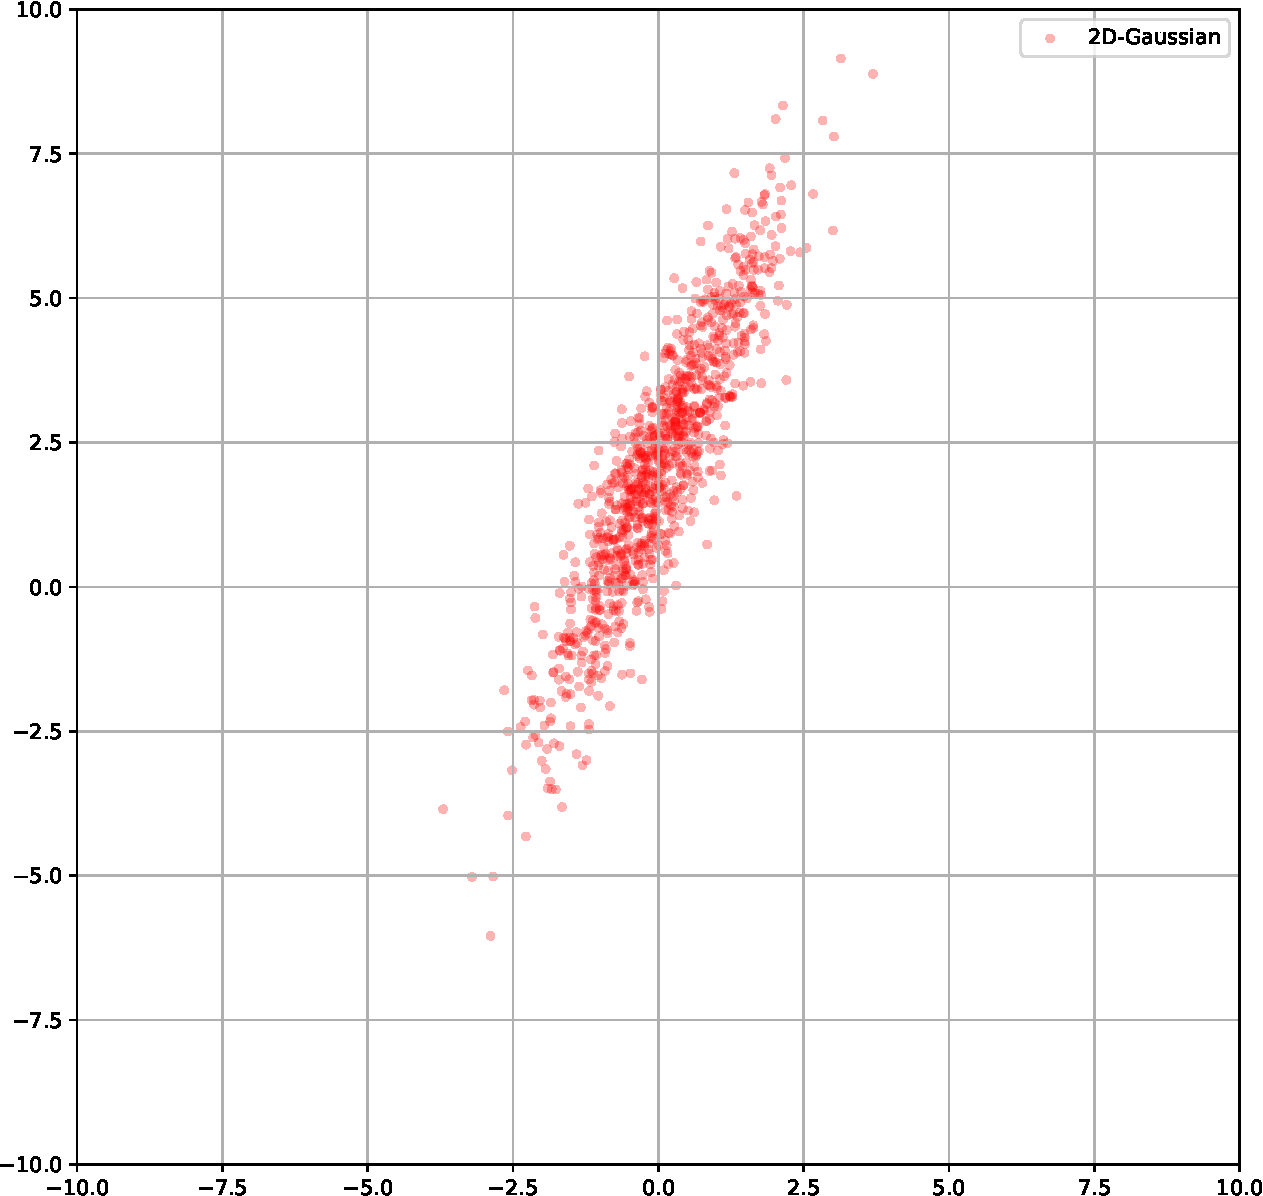
\includegraphics[width=0.55\textwidth]{./assist/figure4.1.pdf}
            \caption{the 1000 points in $X$ sampled from multivariate Gaussian distribution}
        \end{figure}
By using numpy, we have the estimated mean and covariance. Which is 
\begin{align*}
    mean(X) &= (0.01909265, 2.06052385) \\
    cov(X) &= \begin{bmatrix}
    1.03589238 & 2.06244165 \\
    2.06244165 & 5.08839176
    \end{bmatrix}
\end{align*}

% subsection  (end)
\subsection{}% (fold)
\begin{figure}[htbp!]
    \centering
    \subfigure[x]
    {
        \begin{minipage}[b]{.45\linewidth}
            \centering
            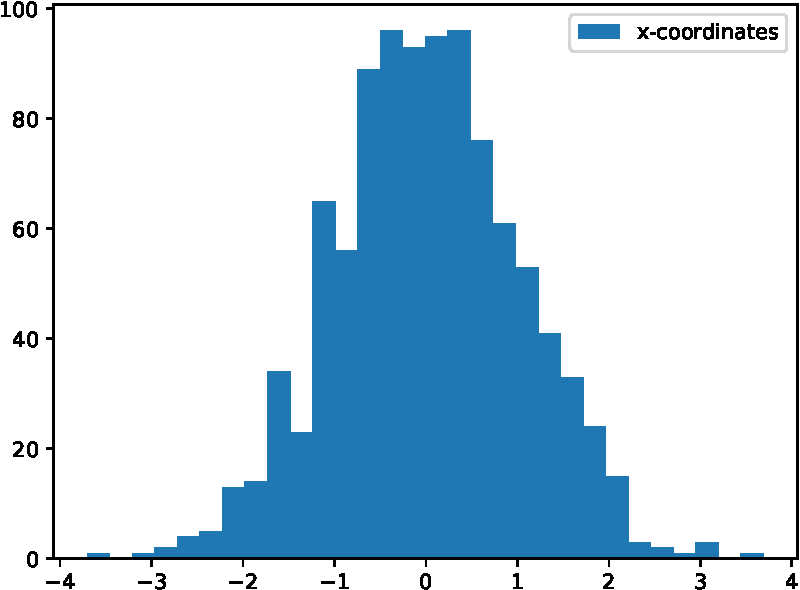
\includegraphics[scale=0.5]{./assist/figure_x_coordinates.pdf}
        \end{minipage}
    }
    \subfigure[y]
    {
        \begin{minipage}[b]{.45\linewidth}
            \centering
            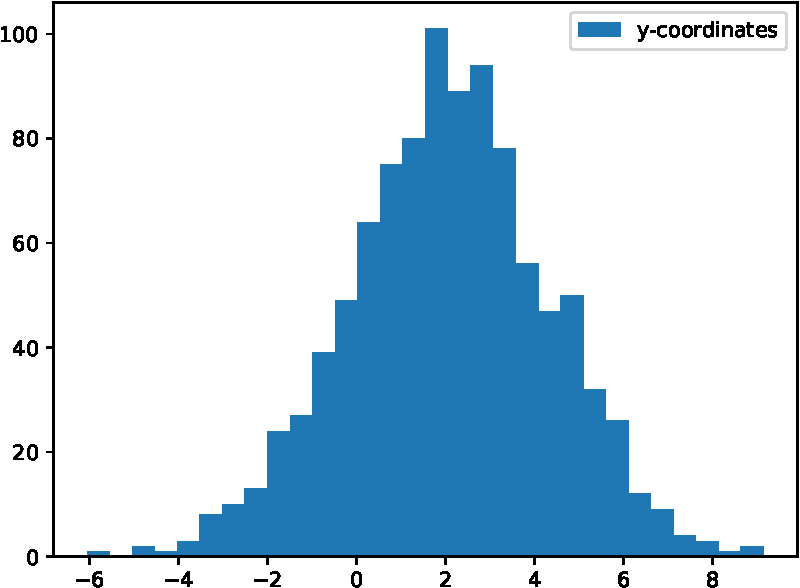
\includegraphics[scale=0.5]{./assist/figure_y_coordinates.pdf}
        \end{minipage}
    }
    \caption{Histogram of x and y coordinates of the 1000 points}
\end{figure}
% subsection  (end)
\subsection{}% (fold)
By the histogram, we can assume the x and y coordinates follow some Gaussian distribution. By using numpy, we get the mean and the variance which is:
\begin{align*}
    \mu_x = 0.019092651459051646 &, \sigma^2_x = 1.0348564864741474 \\
    \mu_y = 2.0605238541899022 &, \sigma^2_y = 5.083303371449154
\end{align*}
% subsection  (end)
\subsection{}% (fold)
\begin{figure}[htbp]
    \begin{center}
        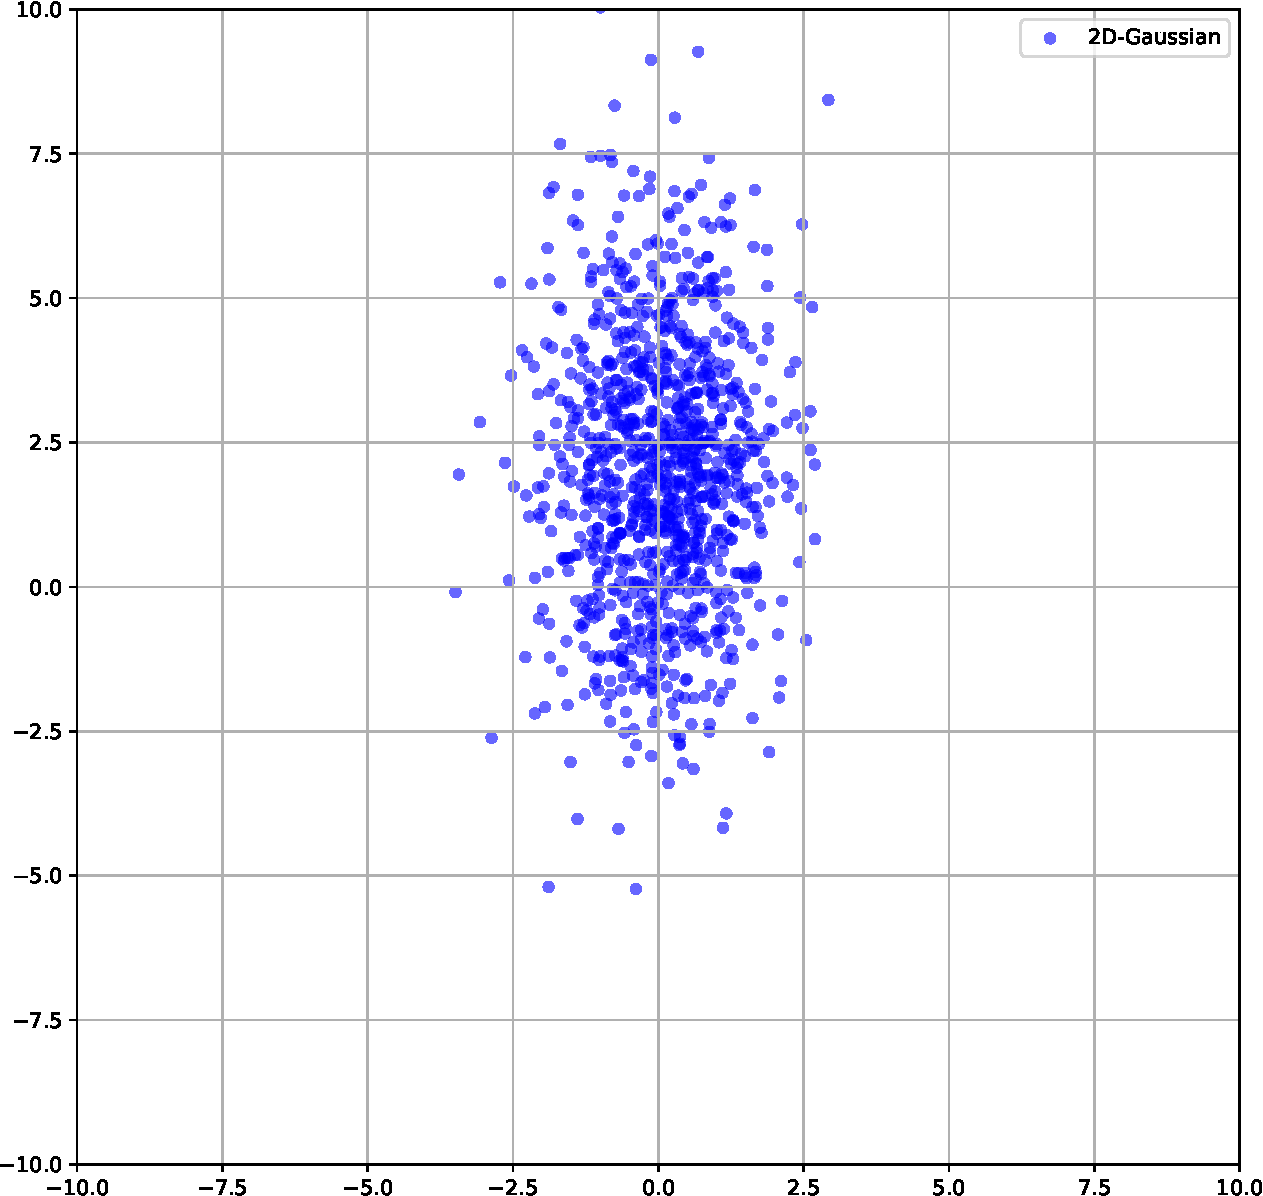
\includegraphics[width=0.75\textwidth]{./assist/figure4.3.pdf}
    \caption{The 2D scatter plot of 1000 points}
    \end{center}
\end{figure}
Difference: New 2D scatter graph is genearlly symmetrical along the y axis, while the original graph is not. The linear relationship between x and y (the covariance is not zero in the first case) lead to the difference.
\clearpage
% subsection  (end)
\subsection{}% (fold)
\begin{figure}[htbp]
    \begin{center}
        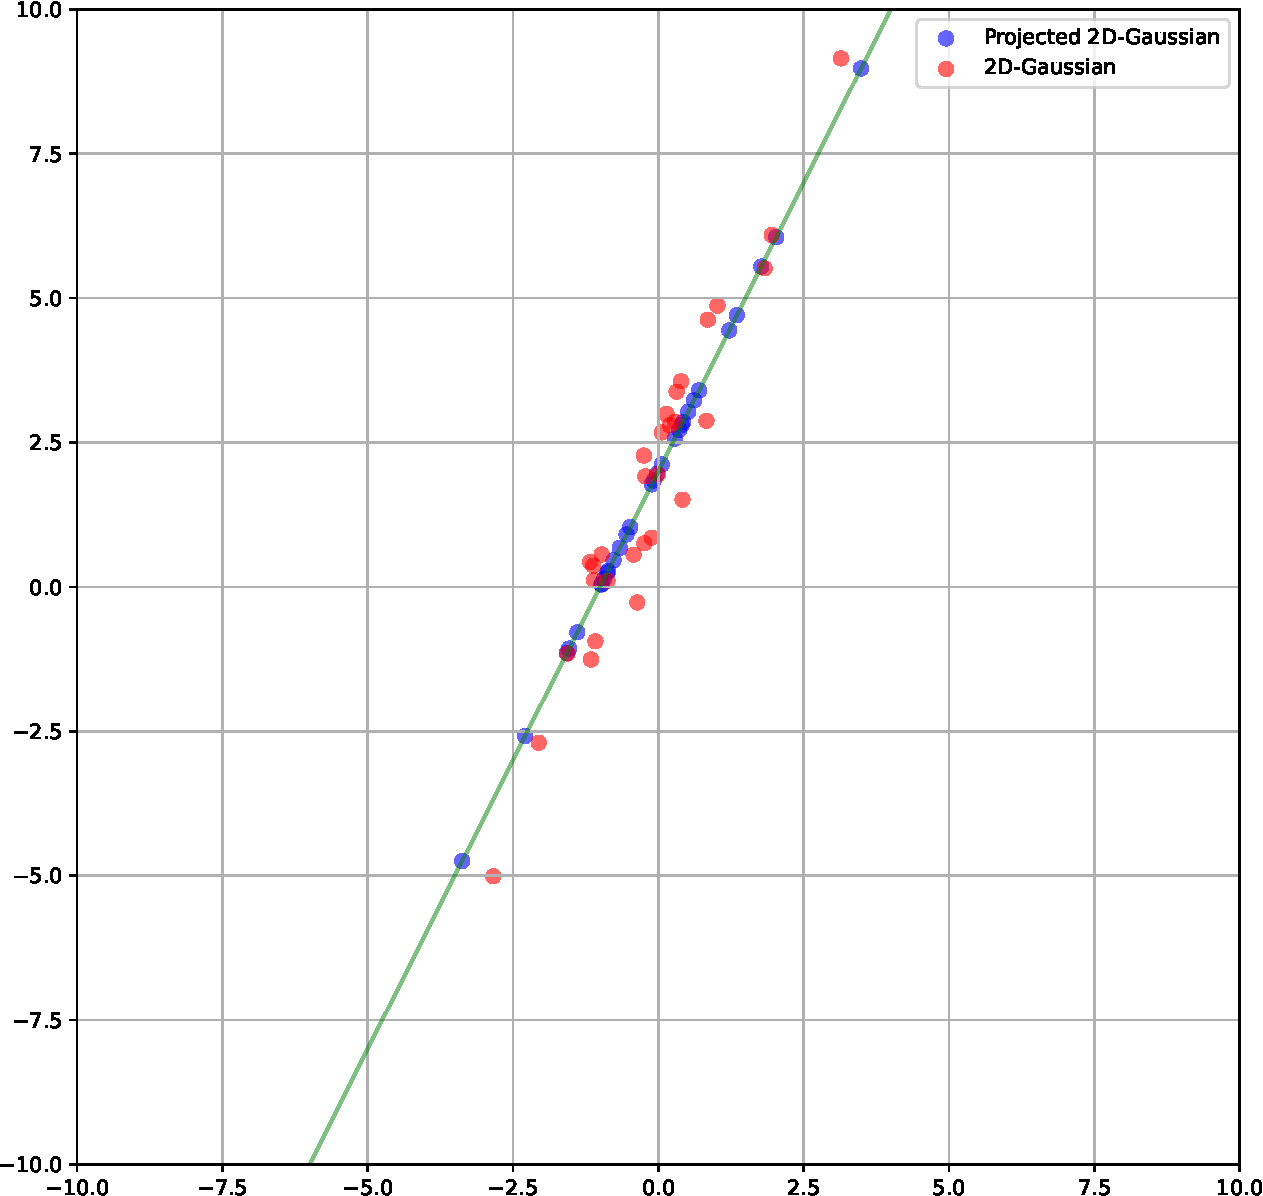
\includegraphics[width=0.43\textwidth]{./assist/figure4.5.pdf}
        \caption{The project points}
    \end{center}
\end{figure}
% subsection  (end)
\subsection{} % (fold)
\begin{figure}[htbp]
    \begin{center}
        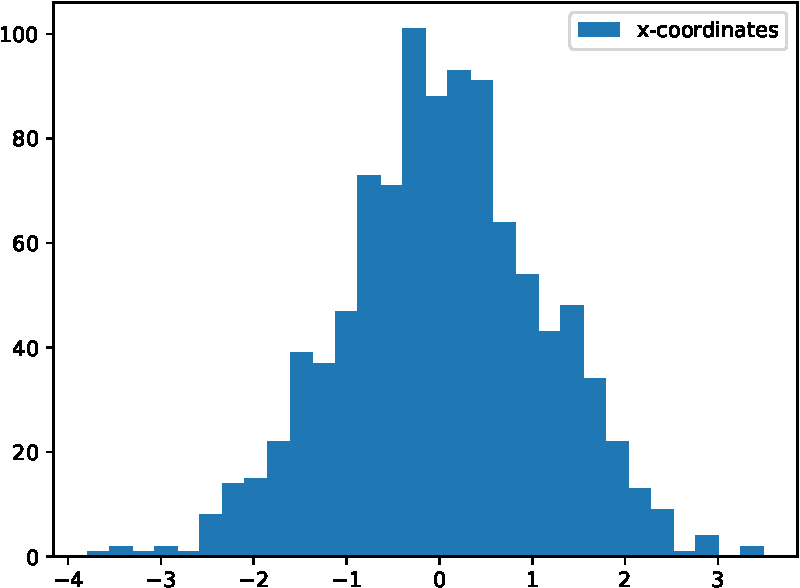
\includegraphics[width=0.5\textwidth]{./assist/figure4.6.pdf}
    \caption{The histogram of the x-coordinates of the projected points}
    \end{center}
\end{figure}
From the histogram, we can assume that the x-coordinates follow some Gaussian distribution. By using numpy, we can get the mean and the variance. Which is:
\begin{align*}
    \mu = 0.028028071967771222, \sigma ^2 = 1.1843834728271614
\end{align*}
% subsection  (end)
% section Density Estimation of Multivariate Gaussian (end)
\section{Matrix/Tensor Transpose}
\subsection{}
Check the corresponding ipynb file.
\subsection{}
We have the transformation below:
\begin{figure}[htbp!]
    \centering
    \subfigure[x]
    {
        \begin{minipage}[b]{.45\linewidth}
            \centering
            
\includegraphics[scale=0.3]{./assist/testimg.jpg}
        \end{minipage}
    }
    \subfigure[y]
    {
        \begin{minipage}[b]{.45\linewidth}
            \centering
            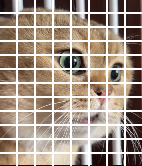
\includegraphics[scale=0.97]{./assist/patched_grid.png}
        \end{minipage}
    }
    \caption{Transformation from (a) to (b)}
\end{figure}
\section{K Means clustering}
\subsection{}
\begin{figure}[h]
    \begin{center}
        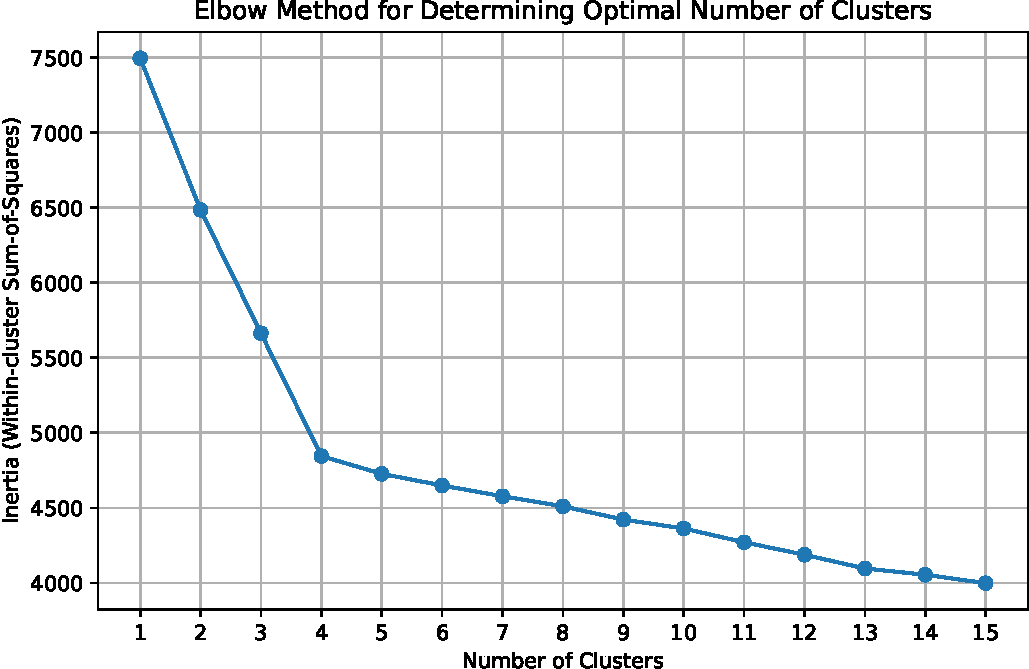
\includegraphics[width=0.5\textwidth]{./assist/elbow_method.pdf}
        \caption{Inertia values corresponding to cluster number}
    \end{center}
\end{figure}
By the figure, we can find that the "elbow" is 4, thus, 4 clusters should be used for this data.
\subsection{}
By setting the cluster number to $4$. We re-apply k-means and there are $25$ observations placed in each cluster, and the value of inertia is $4844.925817623823$.
\subsection{}
\begin{figure}[htbp]
    \begin{center}
        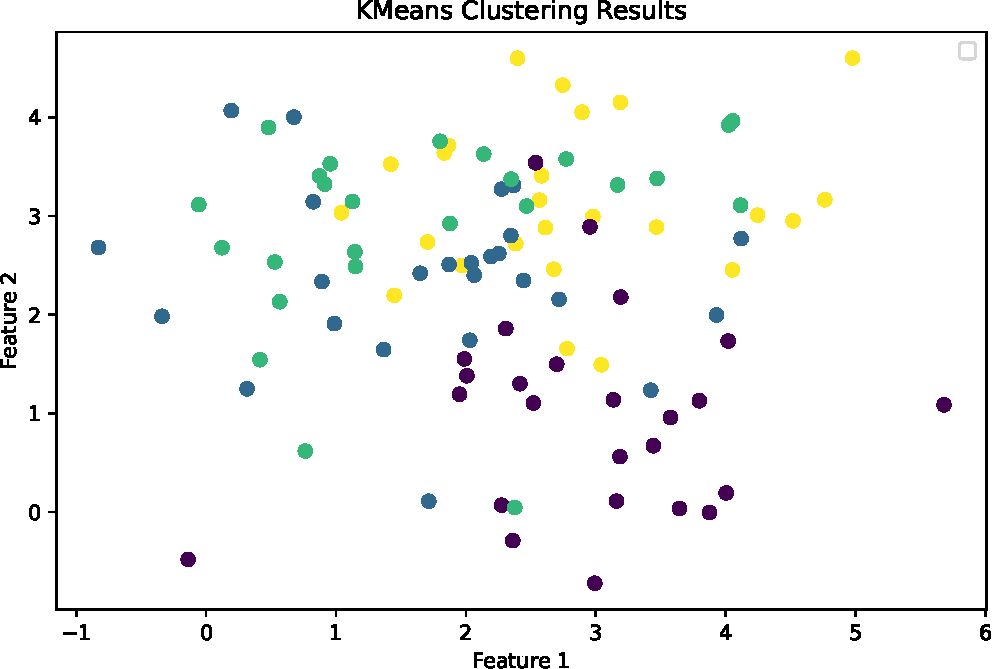
\includegraphics[width=0.5\textwidth]{./assist/kmeans_clustering_results.pdf}
        \caption{KMeans clustering visualization by using first two variables}
    \end{center}
\end{figure}
Based on this plot, it might seemed the clustering is not that accurate. However, this is because we only selected the first two variables to do the visualization while the original data is actually much more complex than that. And we can be sure this is a good choice for the number of centers as this is the elbow point showed in 6.1.
\end{document}
